
\section{Nomenclature}
For ease of the reader, a summary of the notation and mathematical operators used are presented below.
\begin{itemize}
  \item $\Omega$: Mission space.
  \item $\mathcal{O}$: Set of obstacles inside the mission space.
  \item $\mathcal{F}$: Feasible space.
  \item $\mathbf{x}_{a}$: Position of agent $a$.
  \item $r_{a}$: Maximum communication range of agent $a$.
  \item $\hat{p}(\mathbf{x}_{a}, \mathbf{y})$: Local probability of agent $a$ wrt. point $\mathbf{y}$.
  \item $D_{a}$: Communication disk of agent $a$.
  \item $V_{a}$: Visible set of agent $a$.
  \item $U_{a}$: Invisible set of agent $a$.
  \item $\mathcal{B}_{a}$: Neighbors of agent $a$.
  \item $\mathcal{C}_{a}$: Participants in the swarm who are not neighbors of agent $a$.
  \item $\mathbf{X}_{\mathcal{S}}$: Positions of all agents in the swarm $\mathcal{S}$.
  \item $\mathbf{X}_{\mathcal{S}, a}$: Position of participant $a$ in the swarm $\mathcal{S}$.
  \item $\Phi^{n}(\mathbf{X_{\mathcal{S}}}, \mathbf{y})$: Probability of $n$ members in the swarm $\mathcal{S}$ being able to communicate with entity at position $\mathbf{y}$.
  \item $\Phi^{n^{+}}(\mathbf{X_{\mathcal{S}}}, \mathbf{y})$: Probability of $n$ or more members in the swarm $\mathcal{S}$ being able to communicate with entity at position $\mathbf{y}$.
  \item $L(\mathbf{X}_{\mathcal{B}_{a}\cap\{a\}})$: Local probability of coverage for agent $a$.
  \item $D(\mathbf{x}_{a}, \mathbf{x}_{j})$: Proximity of agent $j$ relative to agent $a$.
  \item $H(\mathbf{X}_{\mathcal{B}_{a}\cap\{a\}})$: Local objective for agent $a$. Equal to the local probability of coverage for agent $a$ if active dispersion is not applied.
\end{itemize}
\begin{itemize}
  \item For a set $\mathcal{S}$ defined by $\mathcal{S} = \{s_{0}\hdots s_{N-1}\},\;N<\infty$ the following operators are defined:
  \begin{itemize}
    \item $|\mathcal{S}| = N$: The size of $\mathcal{S}$.
    \item $\mathrm{Comb}(\mathcal{S}, n) = \{\mathcal{A}: \mathcal{A}\subseteq\mathcal{S}, |\mathcal{A}|=n\}$: the set of all subsets of $\mathcal{S}$ of size $n$.
  \end{itemize}
  \item For a set $\mathcal{S}$ of points $\mathbf{x}\in\mathbb{R}^{N}$ defined by $\mathcal{S} = \{\mathbf{x}\in\mathbb{R}^{N}: f(\mathbf{x})\leq\mathbf{0}\}$ the following operators are defined:
  \begin{itemize}
    \item $\delta\mathcal{S} = \{\mathbf{x}\in\mathbb{R}^{N}: f(\mathbf{x}) = \mathbf{0}\}$: The boundary of $\mathcal{S}$.
    \item $\mathrm{int}(\mathcal{S}) = \{\mathbf{x}\in\mathbb{R}^{N}: f(\mathbf{x}) < \mathbf{0}\}$: The interior of $\mathcal{S}$.
    \item $A(\mathcal{S})$: The area of the space bounded by $\delta\mathcal{S}$.
  \end{itemize}
\end{itemize}
\clearpage

\section{System Description}
\subsection{Feasible space}
As in \cite{sun2014escaping}, a \textit{mission space}, $\Omega$, is defined as a simple polygon 
\cite{weissteinsimplepolygon}.
Within the mission space there exists $N_{o}\geq 0$ obstacles, each one of which is defined as a simple polygon.
The set of all obstacles, $\mathcal{O}$, is defined according to \eqref{obstacle_set_def}.
\begin{equation}\label[eq]{obstacle_set_def}
  \mathcal{O} = \begin{cases}
    \{o_{0}\hdots o_{N_{o}-1}\} &, N_{o} > 0\\
    \emptyset &, N_{o} = 0\\
  \end{cases}.
\end{equation}
The obstacles in $\mathcal{O}$ constrains the movement of entities within the mission space, as it is not possible to
penetrate the boundary of an obstacle. Due to this, once an entity is inside $\Omega$, it is constrained to be positioned within
$\Omega$ and outside $\mathrm{int}(o)\;\forall\;o\in\mathcal{O}$. From this the \textit{feasible space}, $\mathcal{F}$, is defined as
all points where it is possible to place an entity:
\begin{equation}\label[eq]{feasible_space_def}
  \mathcal{F} = \{\mathbf{y}\in\mathbb{R}^{2}: \mathbf{y}\in\Omega,\;\mathbf{y}\notin\mathrm{int}(o)\;\forall\;o\in\mathcal{O}\} = \Omega\setminus\bigcup_{o\in\mathcal{O}}\mathrm{int}(o).
\end{equation}

\subsection{Agent}
An \textit{agent} and its properties are defined in a similar manner as in \cite{sun2014escaping}.
An agent, denoted by an index $a$, is defined by its position $\mathbf{x}_{a}\in\mathbb{R}^{2}$ and 
its maximum range of communication $r_{a}$. From this the communication disk of an agent $a$ is defined:
\begin{equation}
  D_{a} = \{\mathbf{y}\in\mathbb{R}^{2}: \norm{\mathbf{x}_{a} - \mathbf{y}}\leq r_{a}\}.
\end{equation}
Assuming line-of-sight (LoS) communication, meaning an agent cannot communicate with an entity if there is 
an obstacle or a mission space wall between them, the \textit{visible set} of agent $a$ is defined:
\begin{equation}\label[eq]{visible_set_def}
  V_{a} = \{\mathbf{y}\in\mathbb{R}^{2}:\mathbf{y}\in D_{a}, \lambda\mathbf{y} + (1-\lambda)\mathbf{x}_{a}\in\mathcal{F}\;\forall\;0\leq\lambda\leq 1\}.
\end{equation}
The counterpart to the visible set, called the invisible set of agent $a$, is simply defined as:
\begin{equation}
  U_{a} = \mathcal{F}\setminus V_{a}.
\end{equation}
An example of the visible set for an agent is shown in \figref{vis_set_example}.

The probability of an agent $a$ being able to communicate with another entity positioned at a point $\mathbf{y}$, from now on called
the local probability of agent $a$ with respect to $\mathbf{y}$, is defined according to:
\begin{equation}\label[eq]{local_prob}
  \hat{p}:\mathbb{R}^{2}\rightarrow [0, 1],\quad\hat{p}(\mathbf{x}_{a}, \mathbf{y}) = \begin{cases}
    p(\norm{\mathbf{x}_{a}-\mathbf{y}}) &, \mathbf{y}\in V_{a}\\
    0 &, \mathbf{y}\in U_{a}
  \end{cases},
\end{equation}
where $p(\cdot)$ is a non-increasing function of its argument.
\begin{figure}[H]
  \centering
  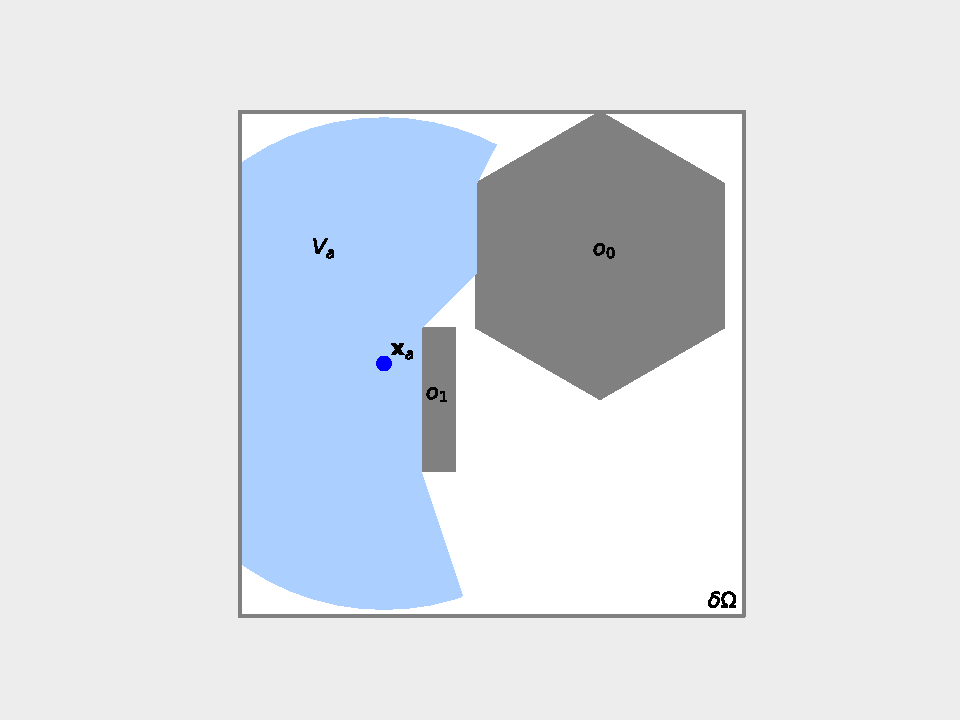
\includegraphics[width=\textwidth]{figs/vis_set_example.pdf}
  \caption{Visible set (light blue) for the agent placed at $\mathbf{x}_{a}$ in a rectangular mission space $\Omega$ with two obstacles ($\mathcal{O} = \{o_{0}, o_{1}\}$)}
  \label[fig]{vis_set_example}
\end{figure}
\subsection{Swarm}
A \textit{swarm} $\mathcal{S}$ of size $N$ is a set of agents $\{a_{0}\hdots a_{N-1}\}$. The state of the swarm is described by the state of its participants, 
and is expressed as a vector $\mathbf{X}_{\mathcal{S}}\in\mathbb{R}^{2N}$ as shown in \eqref{swarm_state_def}.
\begin{equation}\label[eq]{swarm_state_def}
  \mathbf{X}_{\mathcal{S}} = \begin{bmatrix}
    \mathbf{x}_{a_{0}}\\\vdots\\\mathbf{x}_{a_{N-1}}
  \end{bmatrix},\quad\mathbf{X}_{\mathcal{S}, i} = \mathbf{x}_{a_{i}}.
\end{equation}
The maximum radii of communication of the swarm are represented as the vector $\mathbf{r}\in\mathbb{R}^{N}$ as shown in \eqref{swarm_radii_def}.
\begin{equation}\label[eq]{swarm_radii_def}
  \mathbf{r}_{\mathcal{S}} = \begin{bmatrix}
    r_{a_{0}}&\hdots&r_{a_{N-1}}
  \end{bmatrix}^{T}
\end{equation}
\clearpage
In \cite{10.2307/24304959} the probability of success in $x$ out of $n$ independent trials is defined as:
\begin{equation}\label[eq]{independent_success}
  f_{n}(x;\mathbf{p}) = \sum_{\mathcal{A}\in\mathcal{F}_{x}}\Big(\prod_{i\in\mathcal{A}}p_{i}\Big)\Big(\prod_{i\in\mathcal{A}^{c}}1-p_{i}\Big),
\end{equation}
where $\mathbf{p} = \begin{bmatrix}
  p_{0} & \hdots & p_{n-1}
\end{bmatrix}$ and $p_{i}$ denotes the probability of success at the $i$th trial. $\mathcal{F}_{x}$ is equivalent to $\mathrm{Comb}(\{0\hdots n-1\}, x)$, 
and $\mathcal{A}^{c} = \{0\hdots n-1\}\setminus\mathcal{A}$.

Assuming that the distributions for all agents in a swarm $\mathcal{S}$ are independent, \eqref{independent_success} can be used to express 
the probability of $n$ members in the swarm being able to communicate with an entity at a point $\mathbf{y}$:
\begin{equation}\label[eq]{Phi_def}
  \Phi^{n}(\mathbf{X}_{\mathcal{S}}, \mathbf{y}) = \sum_{A\in Comb(\mathcal{S}, n)}\prod_{a\in\mathcal{A}}\hat{p}(\mathbf{x}_{a}, \mathbf{y})\prod_{a\in\mathcal{S}\setminus\mathcal{A}}\big(1-\hat{p}(\mathbf{x}_{a}, \mathbf{y})\big).
\end{equation}
Using \eqref{Phi_def} the probability of \textit{at least} $n$ members in a swarm $\mathcal{S}$ being able to communicate with an entity placed at $\mathbf{y}$ is defined as:
\begin{equation}\label[eq]{more_than_n_prob}
  \Phi^{n^{+}}(\mathbf{X}_{\mathcal{S}}, \mathbf{y}) = 1 - \sum_{i=0}^{n-1}\Phi^{i}(\mathbf{X}_{\mathcal{S}}, \mathbf{y}).
\end{equation}